\documentclass[12pt,a4paper]{report}


\usepackage{mystyle}
\usepackage{pdflscape}

\setcounter{tocdepth}{5}
\setcounter{secnumdepth}{5}

\begin{document}
	\pagenumbering{roman}
	\input{"chapters/title"}
	
	\begin{abstract}
		The problem of cluster geometry optimization is very relevant for many areas from protein structure prediction to the field of nanotechnology. In simple terms, a cluster is an aggregate of interacting atoms or molecules. It can hold a few or even millions of elements. Finding the organization for the \mbox{atoms/molecules} that has the lowest potential energy is an NP-hard problem. In this thesis we proposed an approach based on Swarm Intelligence algorithms. Specifically, we intend to apply an algorithm based on Ant Colony Optimization to the cluster geometry optimization problem, and then compare results with the state-of-art approaches to the same problem. 
	\end{abstract}
	{\bf Keywords:} Cluster geometry optimization, Morse Cluster, Swarm Intelligence, Ant Colony Optimization
	\tableofcontents
	\listoffigures
	\pagenumbering{arabic}
	\input{"chapters/introduction"}
	\input{"chapters/atomic_clusters"}
	\input{"chapters/optimization_of_clusters"}
	\input{"chapters/research_objectives"}
	\input{"chapters/current_work_prel_results"}
	\input{"chapters/conclusions"}
	\appendix
	\chapter{Appendix}
	\begin{landscape}
		\begin{figure}
		  \centering
		  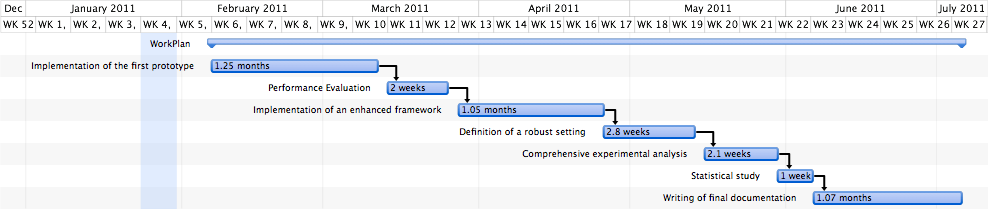
\includegraphics[width=1.5\textwidth]{pictures/WorkPlan}% picture filename
			\caption{WorkPlan}
			\label{fig:WorkPlan}
		\end{figure}
		%\botapic[0.6]{WorkPlan}{Work Plan}
	\end{landscape}
	\bibliographystyle{plain}
	\bibliography{refs}
	
\end{document}

